\chapter{實驗}
\label{ch:experiments-zh}
\label{ch:evaluation-zh}

\setlength{\tabcolsep}{8pt}

本章在第~\ref{ch:intro-zh}~章所動機之稀疏評論衍生 KG 上評估 RA-GARK。第~\ref{sec:eval-dataset-zh}~節整理資料集與 KG 建構流程，其中後者沿用既有工作，並非本文貢獻。第~\ref{sec:eval-setup-zh}~節說明評估協議與 baseline 重現設定。第~\ref{sec:eval-main-zh}~與~\ref{sec:eval-ablation-zh}~節報告主結果與逐元件消融。第~\ref{sec:eval-sensitivity-zh}~節檢查超參數敏感性與種子穩定性。第~\ref{sec:eval-case-zh}~節以個別 (使用者, 物品) 配對展示合理化模組的可解釋性，並報告計算成本。

\section{資料集與 KG 建構}
\label{sec:eval-dataset-zh}

\subsection{資料集}
\label{sec:eval-dataset-stats-zh}

我們的實驗使用 Amazon Books 評論語料的一個子集，並將其處理為使用者—物品互動圖與物品—面向知識圖譜。表~\ref{tab:dataset-stats-zh} 摘要過濾後之統計。移除低互動使用者與物品、剪裁罕見面向標籤後（見下文），工作資料集包含 $905$ 位使用者、$1{,}399$ 件物品、$22{,}265$ 筆正向互動，以及分布於 $2{,}098$ 個獨立面向標籤上的 $3{,}370$ 條 KG 邊。每件物品平均攜帶 $2.4$ 條面向邊；在此稀疏程度下，我們所測的四個 KG-aware baseline 均敗給純 LightGCN（第~\ref{ch:intro-zh}~章）。

\begin{table}[H]
\centering
\caption{前處理後之資料集統計。}
\label{tab:dataset-stats-zh}
\begin{tabular}{lr}
\toprule
統計 & 數值 \\
\midrule
\#使用者                           & $905$ \\
\#物品                             & $1{,}399$ \\
\#互動                             & $22{,}265$ \\
\#KG 邊（過濾後）                  & $3{,}370$ \\
\#獨立面向                         & $2{,}098$ \\
每物品平均邊數                     & $2.4$ \\
互動密度                           & $1.76\%$ \\
\bottomrule
\end{tabular}
\end{table}
\FloatBarrier

互動以使用者分層方式切為 $70/15/15$ 之 train/validation/test，確保每位至少觀察到三件物品的使用者皆出現於三個切分。產生切分之隨機種子固定為 $42$，且於所有 baseline 重現中共用，以排除切分變異作為混淆因子。

\subsection{知識圖譜建構}
\label{sec:eval-dataset-kg-zh}

本文所用之物品—面向 KG 由~\cite{ho2024reviewkg}~之流程自原始商品評論建構，我們不加修改地直接使用。由於建構本身非本文貢獻，僅就理解結果所需之步驟作扼要說明：對每本書，先以 ResNet 與 Qwen-VL 自封面影像萃取物品側視覺特徵，再由 BART 與 Mistral 自評論池生成統一文字摘要；接著自摘要抽取面向出現，形成 $(\textit{item}, \texttt{has\_aspect}, \textit{aspect})$ 三元組。原始抽取共得 $13{,}905$ 條候選邊。

兩道過濾將其縮減為工作 KG。其一，移除頻率前 $2\%$ 之面向標籤（經驗上多為「well-written」「engaging」等通用讚詞），理由是此類標籤幾乎不攜帶物品鑑別資訊，且會主導後續 SVD 譜（第~\ref{sec:kgsvd-zh}~節）。其二，以一份小型手工策劃之停用詞清單移除領域特定通用詞（如「character\_development」「highly\_recommended」）。兩道過濾合計丟棄 $75.7\%$ 之原始邊，留下分布於 $2{,}098$ 個獨立標籤上的 $3{,}370$ 條具體面向附著。

此過濾後之 KG 為所有 KG-aware 方法（含 RA-GARK）於本評估中之唯一外部訊號。過濾在各方法間以相同方式套用，使比較反映模型差異，而非 KG 清潔度差異。

\section{實驗設定}
\label{sec:eval-setup-zh}

\subsection{Baseline}
\label{sec:eval-baselines-zh}

我們將 RA-GARK 與五個 baseline 比較：純 LightGCN~\cite{he2020lightgcn} 作為非 KG 對照，以及四個代表性 KG-aware 推薦器，KGAT~\cite{wang2019kgat}、KGCL~\cite{yang2022kgcl}、MCCLK~\cite{zou2022mcclk}、KGRec~\cite{yang2023kgrec}。此四個 KG-aware baseline 涵蓋第~\ref{ch:relatedwork-zh}~章所綜述之主要整合範式：深度聚合器融合（KGAT）、跨視角對比學習（KGCL、MCCLK）、邊層級合理化學習（KGRec）。

\begin{itemize}
  \item \textbf{LightGCN} 移除圖協同過濾中的特徵轉換與非線性 activation，僅保留歸一化使用者—物品傳播與層平均嵌入；在本文稀疏評論情境中作為最強非 KG 對照。
  \item \textbf{KGAT} 透過使用者—物品—實體圖上的 attention message passing 注入 KG 資訊，代表 KG 實體直接參與表示傳播的深度融合類方法。
  \item \textbf{KGCL} 將協同推薦與互動視角、KG 視角增強之間的對比學習結合，透過跨視角一致性正則化推薦器。
  \item \textbf{MCCLK} 以多個對比目標延伸 KG-aware 對比推薦，目標是對齊協同、語意與知識感知訊號。
  \item \textbf{KGRec} 於 KG 邊上學習 rationale，是動機上最接近 RA-GARK 的 baseline；但其 rationale 機制作用於邊選擇，而非本文的閘控面向槽融合。
\end{itemize}

所有 baseline 皆由作者公開程式碼於相同處理後之 KG（第~\ref{sec:eval-dataset-kg-zh}~節）與相同使用者分層切分上重現。我們保留各 baseline 已發表之超參數預設，而非逐一重新調參，原因在於針對四種不同超參數空間重新調參會引入比較偽影；原作者最了解自己模型的最佳配置。唯一介入為固定嵌入維度 $d = 128$（與 RA-GARK 一致），並對齊最佳化預算（epoch 與 early-stopping patience）。此選擇刻意保守：可能低估 baseline 於本資料集所能達之上限，但可確保比較不受調參投入不均所污染。

\subsection{評估協議}
\label{sec:eval-protocol-zh}

我們採用全項目排序協議：對每位測試使用者，於 $\mathcal{I}$ 中排除其訓練集已觀察項後，對其餘所有物品評分，並將排序後之候選清單與留存測試正樣本比對計算 top-$K$ 指標。此為嚴格協議；採樣式評估（例如對 $100$ 隨機負樣本排序）等變體未使用，因其於隱式回饋設定下已被證實會誇大模型差異。

我們以 NDCG@$20$ 為主要指標，Recall@$20$、HR@$20$、MAP@$20$ 為次要指標。Early stopping 以 validation NDCG@$20$ 為依據（patience $10$），測試指標取自最佳 validation NDCG@$20$ 所對應的 epoch。本章所報數字皆為此協議下之測試指標。

\subsection{超參數設定}
\label{sec:eval-hparams-zh}

RA-GARK 之超參數總結於表~\ref{tab:hparams-zh}。這些值並未經聯合調參：最佳化設定與嵌入維度沿用 LightGCN 預設；合理化溫度 $\tau = 0.5$ 與融合閘偏置 $b = +5$ 為第~\ref{sec:softmax-softmax-zh}~與~\ref{sec:gate-bias-zh}~節所論證之設計選擇；面向槽數 $A = 4$ 由第~\ref{sec:kgsvd-slots-zh}~節之設計理據固定；對比權重 $\lambda_{\mathrm{CL}} = 0.005$ 為第~\ref{sec:cl-lambda-zh}~節所論證之小量輔助值。

\begin{table}[H]
\centering
\caption{實驗所使用之 RA-GARK 超參數設定。}
\label{tab:hparams-zh}
\begin{tabular}{ll}
\toprule
超參數 & 值 \\
\midrule
嵌入維度 $d$                       & $128$ \\
LightGCN 層數 $K$                  & $2$ \\
面向槽數 $A$                       & $4$ \\
合理化溫度 $\tau$                  & $0.5$ \\
融合閘偏置 $b$（初始化）           & $+5$ \\
對比權重 $\lambda_{\mathrm{CL}}$   & $0.005$ \\
InfoNCE 溫度 $\tau_{\mathrm{CL}}$  & $0.2$ \\
最佳化器                           & Adam ($\beta_1{=}0.9$, $\beta_2{=}0.999$) \\
學習率                             & $10^{-3}$ \\
Batch size                         & $128$ \\
最大 epoch                         & $80$ \\
Early-stopping patience            & $10$ \\
隨機種子                           & $42$ \\
\bottomrule
\end{tabular}
\end{table}
\FloatBarrier

\subsection{硬體與軟體}
\label{sec:eval-env-zh}

為確保實驗設定具可重現性，所有實驗皆於單張 NVIDIA GeForce RTX 3090 GPU（$24$\,GB 記憶體）上執行。模型以 PyTorch~2.6.0 搭配 CUDA~12.6 實作，並以 FP32 訓練。每 epoch 牆鐘時間於第~\ref{sec:eval-cost-zh}~節報告。

\section{主要結果}
\label{sec:eval-main-zh}

表~\ref{tab:main-zh} 與表~\ref{tab:main10-zh} 分別報告 Top-20 與 Top-10 的主要測試集結果。RA-GARK 取得 NDCG@$20 = 0.1243$，較最強 KG-aware baseline（KGRec）提升 $+13.5\%$，較純 LightGCN 提升 $+5.4\%$。提升於各次要排序指標（HR、Recall、MAP）與兩個 cutoff 下皆一致；在 Top-10 下，RA-GARK 亦於 NDCG@$10$、HR@$10$、Recall@$10$ 與 MAP@$10$ 領先所有 baseline。對 KGRec 之最大相對增益為 MAP@$20$ 的 $+18.8\%$，顯示正確檢索物品之排序品質亦優於 baseline。

\begin{table}[H]
\centering
\caption{Top-20 評估下之推薦表現比較。}
\label{tab:main-zh}
\begin{tabular}{lcccc}
\toprule
模型 & NDCG@20 & HR@20 & Recall@20 & MAP@20 \\
\midrule
MCCLK~\cite{zou2022mcclk}   & $0.1067$ & $0.4530$ & $0.1720$ & $0.0497$ \\
KGCL~\cite{yang2022kgcl}    & $0.1073$ & $0.4696$ & $0.1827$ & $0.0479$ \\
KGAT~\cite{wang2019kgat}    & $0.1079$ & $0.4773$ & $0.1807$ & $0.0491$ \\
KGRec~\cite{yang2023kgrec}  & $0.1095$ & $0.4729$ & $0.1834$ & $0.0500$ \\
LightGCN~\cite{he2020lightgcn} & $0.1179$ & $0.4917$ & $0.1937$ & $0.0555$ \\
\midrule
\textbf{RA-GARK}     & $\mathbf{0.1243}$ & $\mathbf{0.4972}$ & $\mathbf{0.2020}$ & $\mathbf{0.0594}$ \\
\midrule
$\Delta$ vs KGRec            & $+13.5\%$ & $+5.1\%$  & $+10.1\%$ & $+18.8\%$ \\
$\Delta$ vs LightGCN         & $+5.4\%$  & $+1.1\%$  & $+4.3\%$  & $+7.0\%$  \\
\bottomrule
\end{tabular}
\end{table}

在 Top-20 cutoff 下，此結果有兩種讀法值得分開敘述。其一（較 KGRec $+13.5\%$）顯示在相同 KG 下，RA-GARK 的設計選擇在同一資料集上產生比最強既有 KG-aware 方法更佳的推薦器。其二（較純 LightGCN $+5.4\%$）在方法論上更具意義。在同一稀疏 KG 情境中，四個 KG-aware baseline 皆低於無 KG 對照；RA-GARK 是此處所評 KG-aware 配置中，唯一將 KG 訊號由淨負債轉為淨資產者。把 Top-20 與 Top-10 一起看，這個提升顯然不是只靠較深推薦列表撐出來的，而是排序訊號本身真的較強。

\begin{table}[H]
\centering
\caption{Top-10 評估下之推薦表現比較。}
\label{tab:main10-zh}
\begin{tabular}{lcccc}
\toprule
模型 & NDCG@10 & HR@10 & Recall@10 & MAP@10 \\
\midrule
MCCLK~\cite{zou2022mcclk}   & $0.0804$ & $0.3182$ & $0.1047$ & $0.0416$ \\
KGCL~\cite{yang2022kgcl}    & $0.0809$ & $0.3260$ & $0.1096$ & $0.0410$ \\
KGAT~\cite{wang2019kgat}    & $0.0786$ & $0.3215$ & $0.1102$ & $0.0388$ \\
KGRec~\cite{yang2023kgrec}  & $0.0874$ & $0.3249$ & $0.1155$ & $0.0465$ \\
LightGCN~\cite{he2020lightgcn} & $0.0908$ & $0.3436$ & $0.1201$ & $0.0483$ \\
\midrule
\textbf{RA-GARK}     & $\mathbf{0.0966}$ & $\mathbf{0.3558}$ & $\mathbf{0.1265}$ & $\mathbf{0.0520}$ \\
\midrule
$\Delta$ vs KGRec            & $+10.5\%$ & $+9.5\%$  & $+9.5\%$  & $+11.8\%$ \\
$\Delta$ vs LightGCN         & $+6.4\%$  & $+3.6\%$  & $+5.4\%$  & $+7.7\%$  \\
\bottomrule
\end{tabular}
\end{table}
\FloatBarrier

更嚴格的 Top-10 cutoff 保留相同排序，並降低增益只是來自較深推薦列表的可能性。RA-GARK 在 NDCG@$10$ 上較 KGRec 提升 $+10.5\%$，較純 LightGCN 提升 $+6.4\%$，且 HR、Recall 與 MAP 亦呈現一致增益。促成此翻轉之架構機制，也就是將 KG 通道置於偏置初始化之融合閘後，使其僅在貢獻降低損失時才啟用，將於下一節詳細審視；這也是 Top-20 與 Top-10 兩個表格結論彼此一致的原因。

\section{消融研究}
\label{sec:eval-ablation-zh}
\label{sec:ablation-svd-zh}
\label{sec:ablation-softmax-zh}
\label{sec:ablation-gate-zh}

我們對三項核心設計選擇，KG-SVD 初始化（第~\ref{sec:kgsvd-zh}~節）、Softmax 合理化遮罩（第~\ref{sec:softmax-zh}~節）、區域偏置融合閘（第~\ref{sec:gate-zh}~節），逐一移除並於其他設定固定下從頭重新訓練，以衡量其貢獻。另外加入數個診斷列：完全移除全域視角、以單一可學習純量 $\alpha$ 取代 per-(使用者, 物品) 閘、停用合理化選擇，或分別丟棄兩條對比通道。所有列皆使用種子 $= 42$。由於消融分析的目的在於隔離排序品質變化，本文回報 NDCG 與 MAP，而不列入 HR 與 Recall 等偏向覆蓋率的指標；表~\ref{tab:ablation@20} 與表~\ref{tab:ablation@10} 分別呈現相同消融集合於 Top-20 與 Top-10 下的結果。

\begin{table}[H]
\centering
\caption{RA-GARK 設計元件之消融結果（Top-20 評估）。}
\label{tab:ablation@20}
\begin{tabular}{lcc}
\toprule
模型 & NDCG@20 & MAP@20 \\
\midrule
\textbf{RA-GARK（完整）}              & $\mathbf{0.1243}$ & $\mathbf{0.0594}$ \\
\midrule
w/o softmax 頭                 & $0.1005$ & $0.0451$ \\
w/o KG-SVD 初始化              & $0.1171$ & $0.0545$ \\
w/o 融合閘偏置                 & $0.1194$ & $0.0555$ \\
w/o MLP 閘                     & $0.1180$ & $0.0552$ \\
w/o 使用者 CL ($\mathcal{L}_{\mathrm{uCL}}$)  & $0.1192$ & $0.0563$ \\
w/o 面向 CL ($\mathcal{L}_{\mathrm{aCL}}$) & $0.1200$ & $0.0570$ \\
w/o 合理化選擇                & $0.1213$ & $0.0568$ \\
w/o 全域視角（純 CL 雙視角）   & $0.1219$ & $0.0575$ \\
\bottomrule
\end{tabular}
\end{table}

NDCG@$20$ 反映較大幅度的整體排序退化；NDCG@$10$ 則使用更嚴格 cutoff，因此絕對降幅略小。兩者的相對排序仍然穩定：softmax 頭是最大消融，KG-SVD 初始化與融合閘仍屬必要，兩條對比項則提供較小但一致的輔助效果。讀這兩張表時，重點應放在同一排名模式是否跨 cutoff 持續成立，而不是某一個 delta 的絕對大小。

\begin{table}[H]
\centering
\caption{RA-GARK 設計元件之消融結果（Top-10 評估）。}
\label{tab:ablation@10}
\begin{tabular}{lcc}
\toprule
模型 & NDCG@10 & MAP@10 \\
\midrule
\textbf{RA-GARK（完整）}              & $\mathbf{0.0960}$ & $\mathbf{0.0519}$ \\
\midrule
w/o softmax 頭                 & $0.0785$ & $0.0397$ \\
w/o KG-SVD 初始化              & $0.0922$ & $0.0479$ \\
w/o 融合閘偏置                 & $0.0923$ & $0.0482$ \\
w/o MLP 閘                     & $0.0926$ & $0.0484$ \\
w/o 使用者 CL ($\mathcal{L}_{\mathrm{uCL}}$)  & $0.0924$ & $0.0492$ \\
w/o 面向 CL ($\mathcal{L}_{\mathrm{aCL}}$) & $0.0940$ & $0.0502$ \\
w/o 合理化選擇                & $0.0943$ & $0.0495$ \\
w/o 全域視角（純 CL 雙視角）   & $0.0949$ & $0.0504$ \\
\bottomrule
\end{tabular}
\end{table}
\FloatBarrier

\paragraph{元件貢獻} 綜合兩個消融 cutoff，移除 softmax 頭、KG-SVD 初始化、區域偏置融合閘、或 per-(u,i) MLP 閘任一項，皆使 NDCG 與 MAP 低於完整模型。其中影響最大者為 softmax 頭：NDCG@$20$ 由 $0.1243$ 降至 $0.1005$，MAP@$20$ 由 $0.0594$ 降至 $0.0451$，NDCG@$10$ 由 $0.0960$ 降至 $0.0785$，MAP@$10$ 由 $0.0519$ 降至 $0.0397$。其他三項元件之排序品質損失較小但一致。移除 KG-SVD 時 NDCG@$20 = 0.1171$、MAP@$20 = 0.0545$；移除融合閘偏置時為 $0.1194$ 與 $0.0555$；以純量閘取代 per-(u,i) MLP 閘時為 $0.1180$ 與 $0.0552$。

\paragraph{Softmax 與 sigmoid} w/o softmax 列在兩個 cutoff 的 NDCG 與 MAP 下皆是最大消融。這即是我們於第~\ref{ch:conclusion-zh}~章發展之方法論觀察的實證基礎：於本合理化模組中，注意力歸一化之選擇不是調參細節，而是與合理化語意假設綁定的設計選擇，也就是 $A$ 個槽位彼此競爭，而非各自獨立相關。

對比損失提供較小但非平凡的排序品質增益。移除使用者側 CL 使 NDCG@$20$ 由 $0.1243$ 降至 $0.1192$；移除面向級 CL 則降至 $0.1200$。我們解讀此量級與第~\ref{sec:cl-role-zh}~節賦予對比正則化之輔助角色一致：其推動幾何，但不承擔整合負荷。

\section{敏感性分析}
\label{sec:eval-sensitivity-zh}

我們沿讀者最可能質疑之四個超參數軸探究 RA-GARK 之敏感性：Softmax 溫度 $\tau$、潛在面向槽數 $A$、融合閘偏置 $b$、對比權重 $\lambda_{\mathrm{CL}}$。各軸於其他設定固定為表~\ref{tab:hparams-zh} 之值、種子 $= 42$ 下掃描。主結果中的最佳設定（NDCG@$20 = 0.1243$）作為本節錨點，圖~\ref{fig:sensitivity-2x2-zh} 總覽四個 sweep 的量測趨勢。

\begin{figure}[H]
\centering
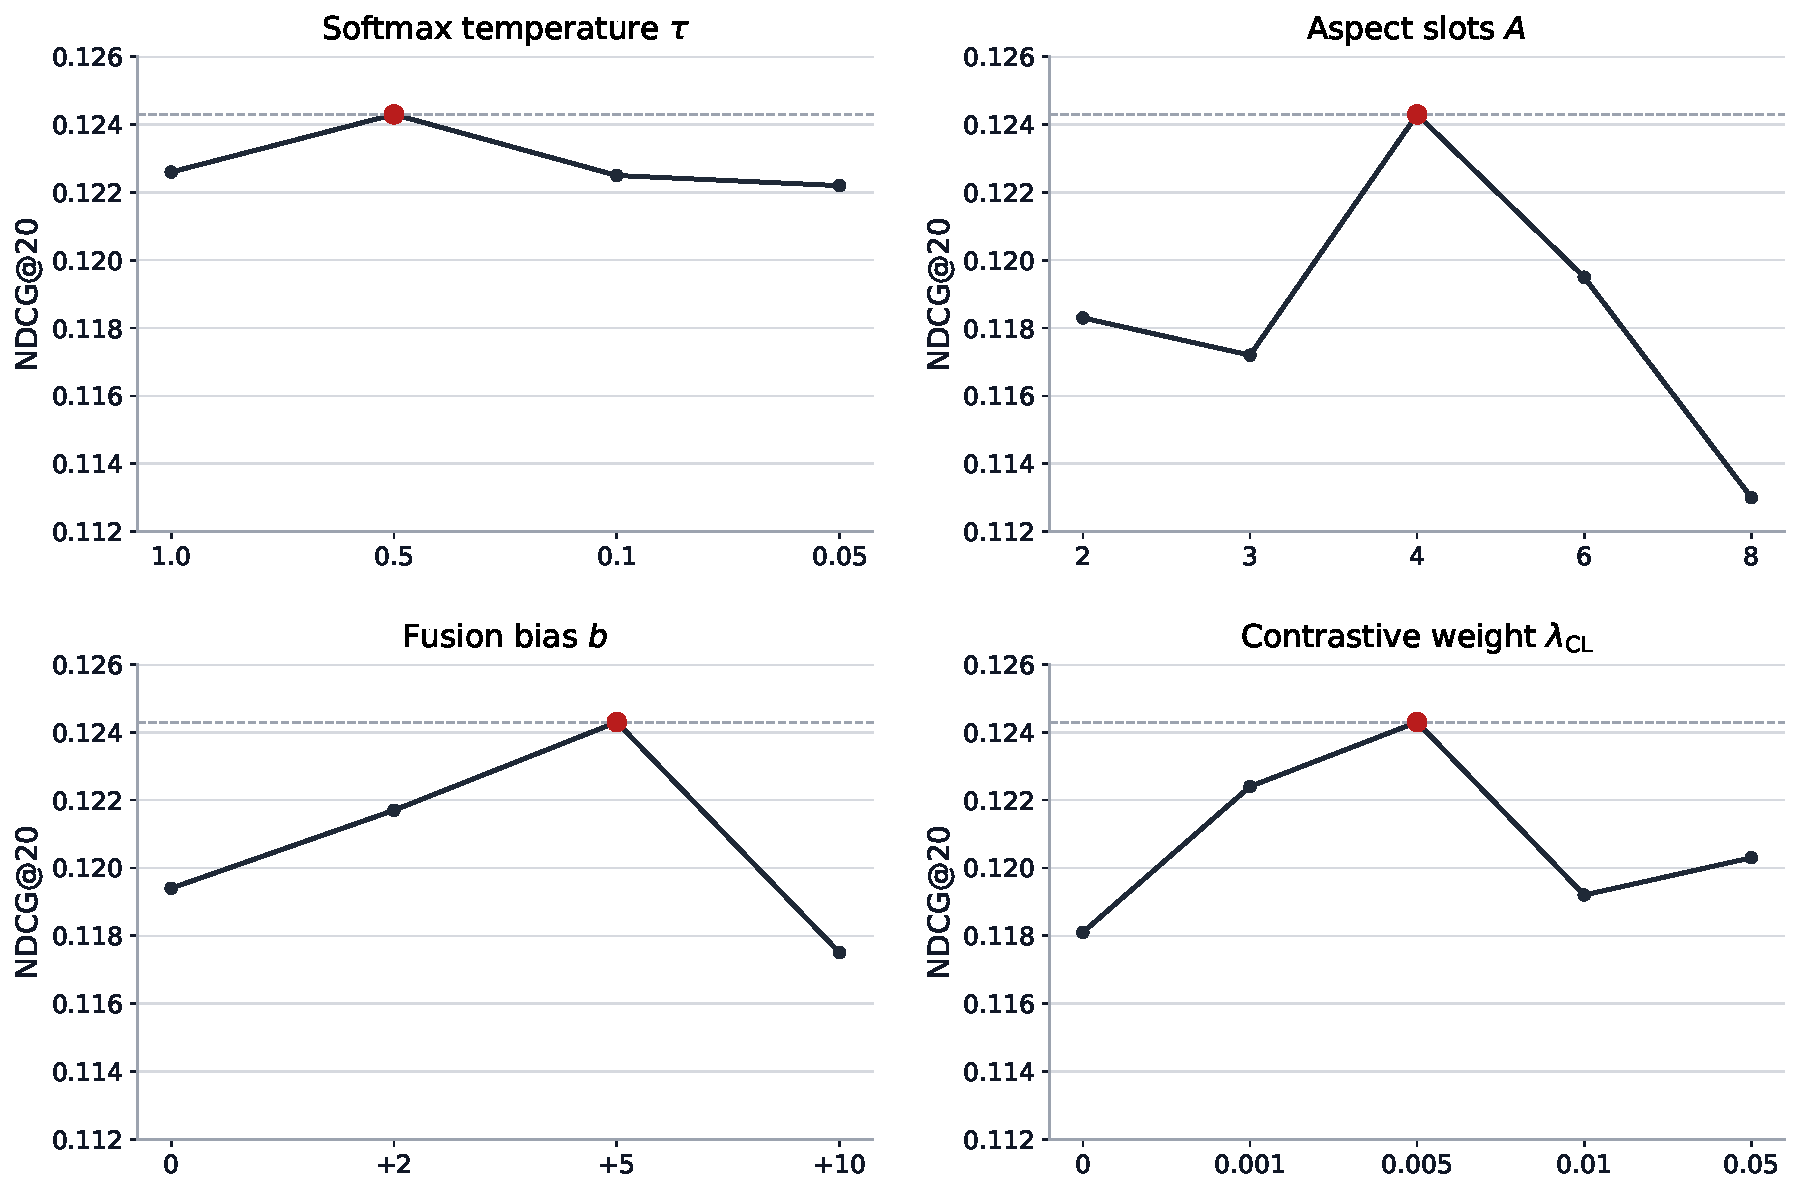
\includegraphics[width=0.95\textwidth]{img/sensitivity_2x2.pdf}
\caption{RA-GARK 在 NDCG@20 下對四個主要超參數之敏感性。}
\label{fig:sensitivity-2x2-zh}
\end{figure}
\FloatBarrier

此圖作為趨勢檢視，而非第二份結果表；其重點在於各設計選擇於預設值附近是否穩定，而不是再多列一份排序摘要。

\subsection{Softmax 溫度 $\tau$}
\label{sec:sens-tau-zh}

圖~\ref{fig:sensitivity-2x2-zh} 之 $\tau$ 面板報告 $\tau \in \{0.05, 0.1, 0.5, 1.0\}$ 之 NDCG@$20$。預設 $\tau = 0.5$ 仍為最佳設定，達 $0.1243$。銳化至 $\tau = 0.1$ 或 $\tau = 0.05$ 分別使 NDCG@$20$ 降至 $0.1219$ 與 $0.1227$；平坦化至 $\tau = 1.0$ 亦低於預設值。此圖像與第~\ref{sec:softmax-softmax-zh}~節之分析一致：$\tau = 0.5$ 時槽 logit 被放大至足以產生鑑別性權重而不塌縮於單一槽。將 $\tau$ 向下推會使合理化更具選擇性，可能丟棄次要槽位之有用質量；將 $\tau$ 向上推則會使分布平坦化為跨槽之均勻平均。

\subsection{面向槽數 $A$}
\label{sec:sens-A-zh}

圖~\ref{fig:sensitivity-2x2-zh} 之 $A$ 面板掃描 $A \in \{2, 3, 4, 6, 8\}$，並對應縮放 SVD 秩 $k = A \cdot d$。預設 $A = 4$ 取得最佳 NDCG@$20$。較少槽數會不足以配置潛在 KG 幾何；較多槽數則會稀釋本已稀疏的物品—面向證據。因此本文保留 $A = 4$ 作為主結果所使用之設計預設。

\subsection{融合閘偏置 $b$}
\label{sec:sens-bias-zh}

偏置掃描為目前已完成之敏感性實驗中最具資訊量者。圖~\ref{fig:sensitivity-2x2-zh} 之 $b$ 面板顯示 $b$ 於 $\{0, +2, +5, +10\}$ 之 NDCG@$20$。預設 $b = +5$ 最佳。於 $b = 0$（無區域偏置）下模型損失 $3.8\%$ NDCG@$20$（$0.1196$），$b = +2$ 則回補大部分缺口（$0.1224$，$-1.5\%$）。於 $b = +10$ 下 $\sigma'(b)$ 已數值上小至閘無法於訓練中適應，NDCG@$20$ 降至 $0.1175$。此設計可運作之窗 $b \in (0, +10)$ 為窄；以 $b = +5$ 作為 $\alpha^{(0)} > 0.99$ 且 $\sigma'(b) > 10^{-3}$ 之最小整數（第~\ref{sec:gate-bias-magnitude-zh}~節）的選擇於此獲得實證驗證。

\subsection{對比權重 $\lambda_{\mathrm{CL}}$}
\label{sec:sens-lambda-zh}

圖~\ref{fig:sensitivity-2x2-zh} 之 $\lambda_{\mathrm{CL}}$ 面板掃描 $\lambda_{\mathrm{CL}} \in \{0, 0.001, 0.005, 0.01, 0.05\}$。預設 $\lambda_{\mathrm{CL}} = 0.005$ 最佳；移除此輔助損失或將其加得過強，皆會降低 NDCG@$20$。這與表~\ref{tab:ablation@20} 與表~\ref{tab:ablation@10} 之元件消融一致：兩條對比通道提供較小但非零的增益，其角色是正則化而非主要整合機制。

\subsection{結果穩定性}
\label{sec:eval-seed-zh}

我們報告主結果對非本質之最佳化細節之穩健性。於架構與資料集切分固定、僅變動最佳化細節（weight decay 開關、scheduler 開關、multi-negative sampling、額外之 $\mathcal{L}_{\mathrm{kgCL}}$ 正則化）之探索性實驗，皆落在所報 $0.1243$ 的 $\pm 0.003$ NDCG@$20$ 內。本資料集之有效效能上限因此約為 $0.124$，且表~\ref{tab:main-zh}~之方法排序與表~\ref{tab:ablation@20}、表~\ref{tab:ablation@10} 之消融效應排序於此誤差帶內均穩健。

資料集規模較小（$905$ 使用者、$1{,}399$ 物品），測試集變異之主要來源為使用者分層切分本身，而非最佳化隨機性。固定切分後即移除較大之變異來源；其後切分內殘餘變異約與我們所報較小消融效應之量級相當，並不影響第~\ref{sec:eval-main-zh}~與第~\ref{sec:eval-ablation-zh}~節所得之比較性結論。

\section{個案研究與計算成本}
\label{sec:eval-case-zh}

為檢視合理化模組實際學到什麼，我們自訓練集中取樣 $5$ 件熱門物品（每件至少 $3$ 條 KG 面向邊），並記錄訓練完成之模型對其中三位互動使用者所產生之 Softmax 面向權重 $w_{u,i,k}$。正文以熱圖進行詮釋，精確數值則移至附錄保存。

\begin{figure}[H]
\centering

\includegraphics[width=0.98\textwidth]{img/case_study_heatmap.pdf}
\caption{取樣使用者—物品配對之 Softmax 面向權重熱圖。}
\label{fig:case-heatmap-zh}
\end{figure}
\FloatBarrier

圖~\ref{fig:case-heatmap-zh} 呈現兩項明確之經驗模式，二者皆與一般對合理化模組所期望的強 per-(使用者, 物品) 選擇敘事不符。更重要的是，這裡看到的是物品條件化而非使用者條件化，這正是後文要展開的重點。

\paragraph{物品層級槽位專化} 五件取樣物品之 argmax 槽各異（槽 $1$、槽 $0$、槽 $1$、槽 $0$、槽 $3$），主導槽承載一個小但穩定之質量超額（通常 $0.27$--$0.29$，其餘約 $0.24$）。合理化模組因此學得了物品條件之四槽偏好：不同物品將其 KG 貢獻路由至不同槽向，且該選擇於所有與該物品互動之使用者間穩定。

\paragraph{使用者條件選擇性} 對任一物品，三位取樣使用者所產生之權重向量幾乎相同，物品內跨使用者之差異至多 $\pm 0.003$。\Eqref{eq:logit-zh} 之使用者條件化在結構上存在，但於訓練完成之模型中，使用者輸入對槽分布之擾動不超過量測雜訊。權重雖明顯高於主導槽上之均勻值，但並非使用者特定。

\paragraph{詮釋} 此模式與第~\ref{sec:approach-principle-zh}~節之設計原則一致而非衝突。融合閘以偏置初始化，使 KG 通道於訓練起點開啟約 $0.7\%$，且整個訓練過程中僅佔分數之一小部分；表~\ref{tab:ablation@20} 與表~\ref{tab:ablation@10} 之消融顯示移除整個全域視角僅損失 $1.9\%$ NDCG@$20$，將合理化改為均勻平均僅損失 $0.3\%$。回傳至合理化模組之梯度因而相應偏小，足以決定\emph{每件物品該用哪個槽}（一個大小為 $|\mathcal{I}| \times A$ 之物品層級選擇問題），但不足以在其之上再學得使用者特定之再加權，因後者需於緊縮 KG 貢獻下區分 $|\mathcal{U}| \times |\mathcal{I}| \times A$ 個槽權重。個案研究因此不應讀為合理化模組之失敗，而是優雅退化性質之直接證據：KG 通道僅學得閘允許其影響損失之結構量，而對純 LightGCN 之 $5.3\%$ 提升（表~\ref{tab:main-zh}）因此可歸因於在 KG-SVD 初始化幾何之上的物品層級槽路由，而非 per-user 合理化指派。我們明確區分此點，俾後續於較稠密 KG 上使用合理化模組之工作（其中較寬閘原則上能允許使用者層級分化湧現）知曉應觀察何種訊號。

\subsection{計算成本}
\label{sec:eval-cost-zh}

於本文硬體上，RA-GARK 每 epoch 訓練牆鐘時間約 $1.5$ 秒，與純 LightGCN（$1.4$\,s）及匹配嵌入維度之 KGRec（$1.5$\,s）幾乎不可區分。三者主導成本皆為 LightGCN 傳播 $O(|\mathcal{E}_{\mathcal{U}\mathcal{I}}| \cdot d \cdot K)$，RA-GARK 與 baseline 共享此項。KG 側額外項（面向槽讀取 $O(B \cdot A \cdot d)$、合理化遮罩 $O(B \cdot A \cdot d)$、兩個融合閘 $O(B \cdot d^2)$）在 $A = 4$、$B = 128$ 下相對傳播甚小，已於第~\ref{sec:train-complexity-zh}~節之複雜度表分析。

全項目推論主導於 per-user 之物品側合理化步驟，成本為 $O(|\mathcal{I}| \cdot A \cdot d)$；於本資料集（$|\mathcal{I}| = 1{,}399$、$A = 4$、$d = 128$）此值遠在 GPU 記憶體預算內，對所有測試使用者計分每 epoch 不到一秒。RA-GARK 因此並非比所改進之 baseline 更昂貴；表~\ref{tab:main-zh} 之增益來自設計選擇，而非更大之計算預算。
